\section{系统编码}

\subsection{前后端交互模型}

前后端交互模型如图4.1所示

\begin{figure}[thbp!]
	\centering
	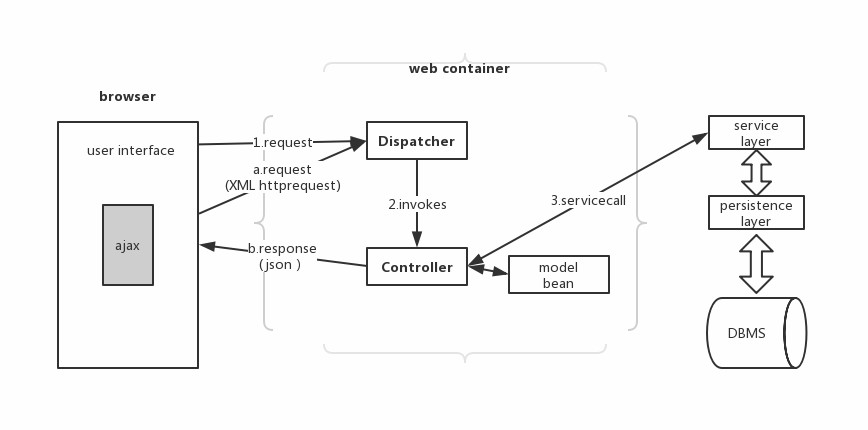
\includegraphics[width=1.0\linewidth]{figure/BS_structure}
	\label{fig:BS_structure}  \\
		4.1 B/S架构图
\end{figure}

\subsubsection{RESTful API}

REST全称是Representational State Transfer,中文意思是表述(编者注:通常译为表征)性状态转移。

RESTful API有以下的特征:

(1)每一个uri代表一种资源。

(2)客户端和服务器之间,传递这种资源的某种表现层。

(3)客户端通过四个HTTP动词(GET、POST、DELETE、PUT),对服务器端资源进行操作,实现"表现层状态转化"(增删改查)。

(4)URL中通常不出现动词,只有名词。

(5)使用JSON不使用XML。

\subsubsection{使用Redux存储网络请求状态}

Redux 是 JavaScript 状态容器,提供可预测化的状态管理。可以让你构建一致化的应用,运行于不同的环境(客户端、服务器、原生应用),并且易于测试。其使用Immutable数据结合React能让页面相应数据进行最小颗粒度的更新DOM结点。

redux数据流如图4.2所示

\begin{figure}[thbp!]
	\centering
	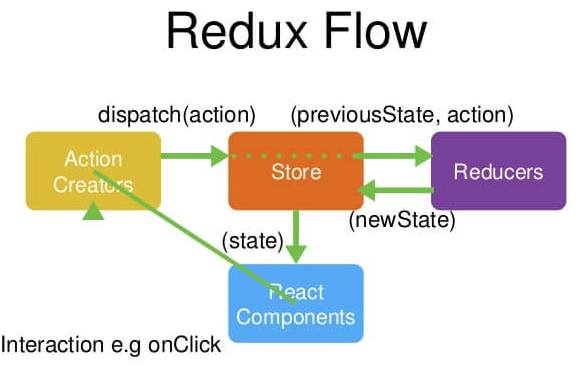
\includegraphics[width=1.0\linewidth]{figure/redux}
	\label{fig:redux} \\
		4.2 redux数据流
\end{figure}

每一次发起http请求获得响应的时候触发一个Redux Action,将服务端返回的数据存储在store中。这样做的好处是所有的需要使用服务端数据的React组件不需要影响父子组件之间的数据流直接提取公用的状态。

\subsection{账号系统}

\subsubsection{密码加密}

用户密码的创建和验证简略代码如下:

\begin{lstlisting}[language=C]
@property
def password(self):
raise TypeError("cannot read a user's password")

@password.setter
def password(self, password):
self.password_hash = generate_password_hash(password)

def verify_password(self, password):
if not password:
return False
return check_password_hash(self.password_hash, password)
\end{lstlisting}

@property装饰器装饰一个属性的getter,修饰的函数名为属性名,返回的值是该属性的getter,此处该属性不能直接访问访问则会抛出异常。

@property同时会全局创建一个@password.setter的装饰器装饰属性的setter,在设置password的时候我们其实设置的是password\_hash这个属性,值为hash加密过的password。

处理登陆请求的时候调用verify\_password函数判断密码是否正确。

这样做的好处就是即使是数据库管理员也不可能知道用户的密码,只能看到加密后的字符串,同时md5是不可逆的加密方式,不能由加密后的字符串反推出明文,保证了数据的机密性。

\subsubsection{邮箱验证}

用户注册和忘记密码的时候需要使用邮箱验证。在用户注册成功后会创建一个用户独有的token,将token作为链接参数发送给用户邮箱中,在用户点击链接进入验证页面的时候会将token返回后端后端进行验证。

验证失败有两种结果,一是token过期,二是token中的用户信息不匹配当前用户。通常不匹配的情况有三种:

(1) 用户自己改了url中的token

(2) 中间商劫持被修改了token信息。

(3) 非法重定向。

无论哪种都是非法篡改token的行为,影响用户信息安全。

邮箱激活流程图如图4.3所示,用户注册以后,系统会向注册时候填写的邮箱中发送一个邮件,里面带有验证地址的连接,用户点击以后进入验证页面。有两种用户,一种是自主创建的用户,一种是管理员批量添加的用户,第二种用户在登陆的时候需要填写邮箱,然后再进行激活。如果用户篡改连接地址或者被运营商劫持验证时不会通过。因为连接中有一个参数为token,token是将用户信息和时间戳hash后的可逆加密字符串,一旦服务端验证token的时候信息和连接中的username参数对不上那就会返回失败。

\begin{figure}[thbp!]
	\centering
	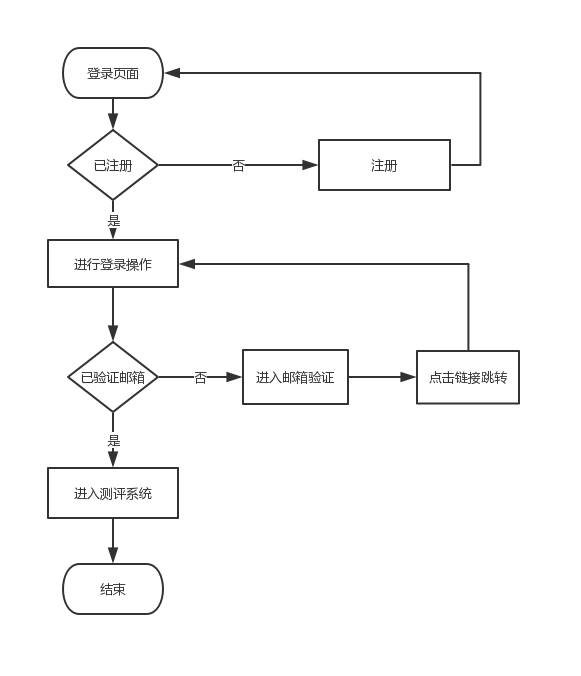
\includegraphics[width=1.0\linewidth]{figure/register_email}
	\label{fig:register_email} \\
		图4.3 注册邮箱激活
\end{figure}

找回密码流程图如图4.4所示,用户忘记密码后点击忘记密码,需要输入自己的用户名,随后系统会向用户名注册时候对应的邮箱发送验证邮箱,点击邮箱中的连接进入验证界面如果验证通过则会出现新密码输入框。

\begin{figure}[thbp!]
	\centering
	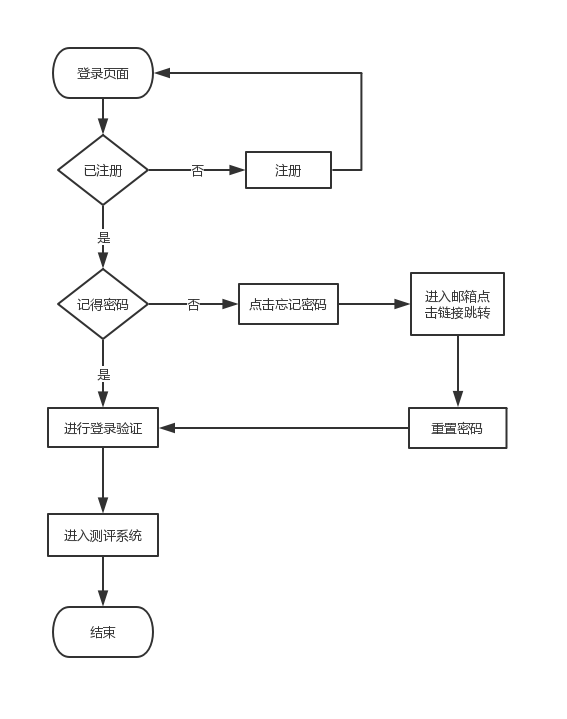
\includegraphics[width=0.8\linewidth]{figure/password_mail}
	\label{fig:password_email} \\
		图4.4 忘记密码邮箱验证
\end{figure}

\subsection{评测与数据分析}

\subsubsection{上传试卷}

示例试卷excel表格如图4.5所示

\begin{figure}[thbp!]
	\centering
	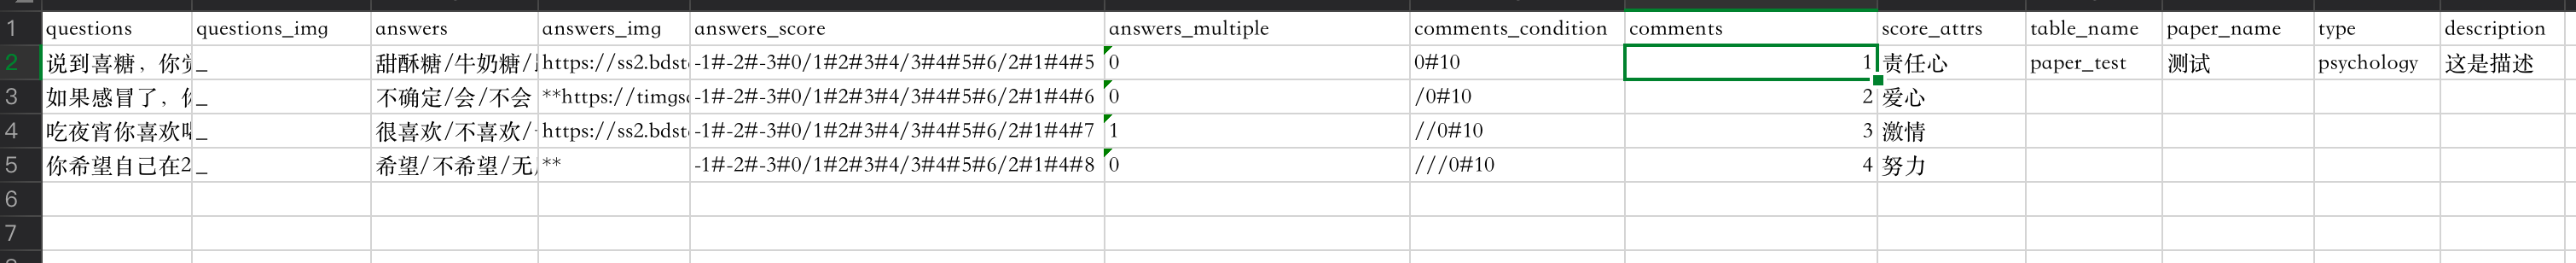
\includegraphics[width=1.0\linewidth]{figure/paper}
	\label{fig:paper} \\
		图4.5 示例试卷
\end{figure}

mysql中试卷表如图4.6所示

\begin{figure}[thbp!]
	\centering
	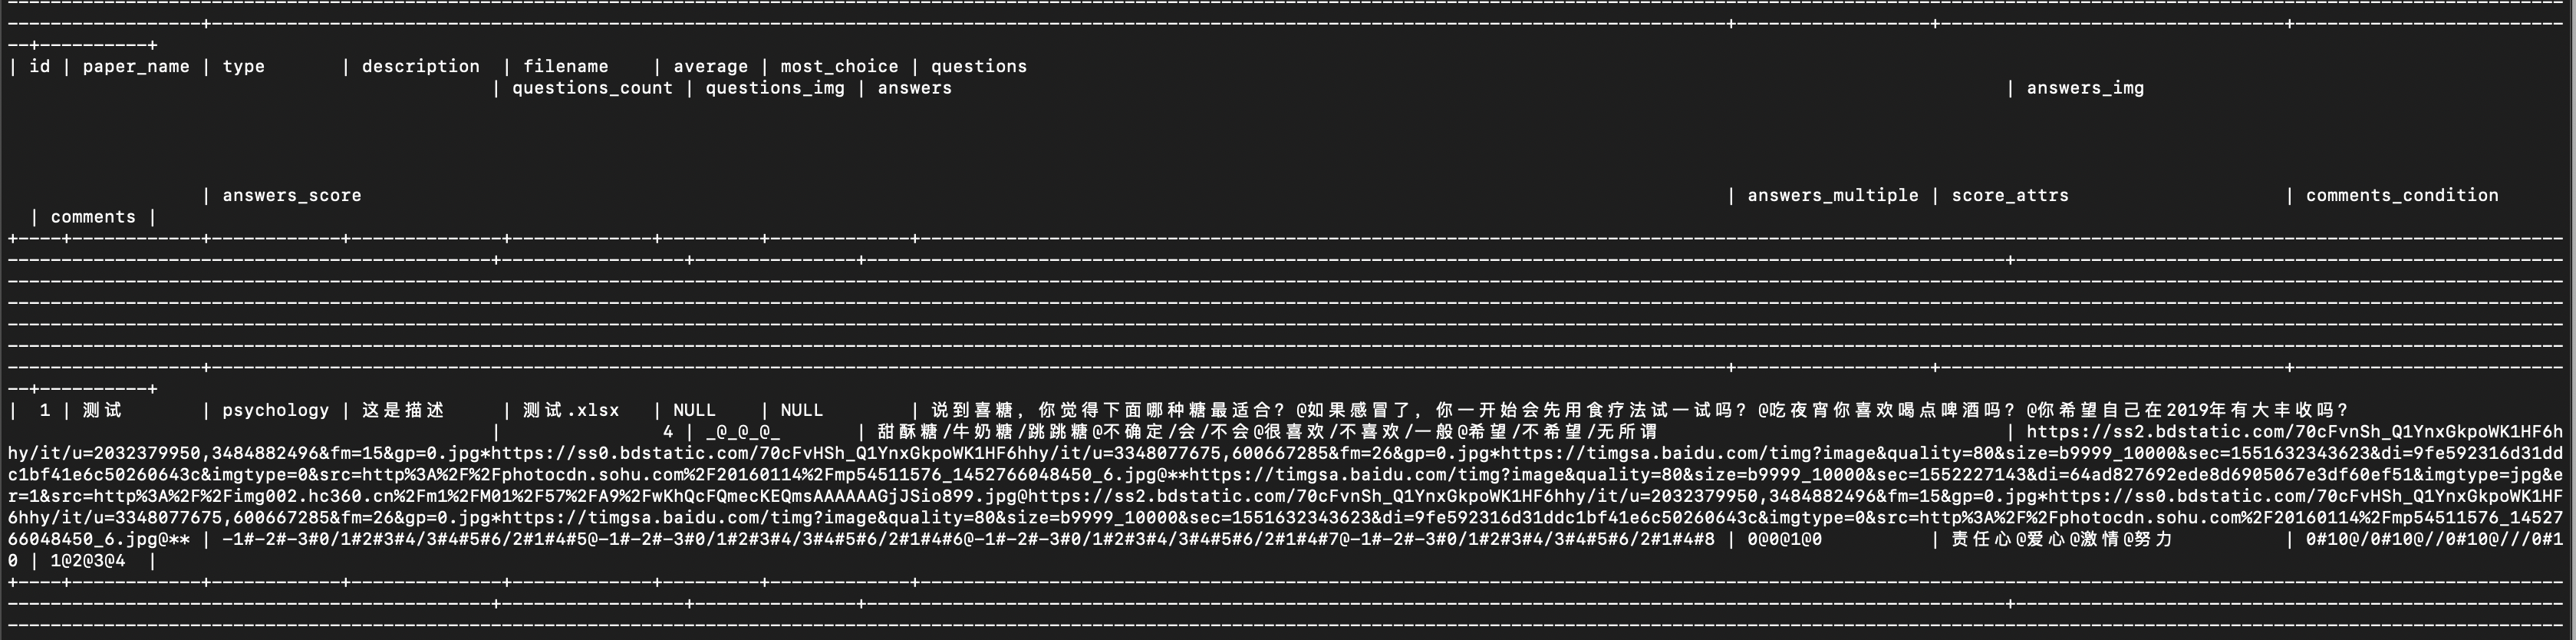
\includegraphics[width=1.0\linewidth]{figure/paper_database}
	\label{fig:paper_database} \\
		图4.6 试卷表
\end{figure}

上传试卷是通过上传excel表格。

questions 问题的题目

questions\_img 题目的配图的图片链接地址

answers 题目的答案,答案之间用"/"来进行分割

answers\_img 题目答案的配图的图片链接地址,配图之间用"*"进行分割,只支持一个答案只有一个配图

answers\_score 对应每个答案对应试卷指标的分数加成,正数为增加,负数为减少,0则表示该答案对此项指标没有影响,每个答案之间用"/"分隔,每个指标之间用"\#"分隔

answers\_multiple 该题目是否是多选,0表示单选,1表示多选

comments\_condition 试卷各种评论的条件,每个指标之间用"/"分隔,0\#10表示该指标大于零小于10

comments 具体的评论内容

score\_attrs 试卷的得分指标

table\_name 数据库中的表名

paper\_name 试卷名称

type 试卷的类型,psychology代表室心理评测,grade代表普通试卷,决定了试卷的算分机制

description 试卷的描述

上传文件后后端通过读取excel表格文件将数据插入到数据库中。

每个问题之间的数据使用"@"来进行连接。

在评测时候后端会对表数据进行解析和构建对象发送给前端。

试卷数据结构如图4.7所示

\begin{figure}[thbp!]
	\centering
	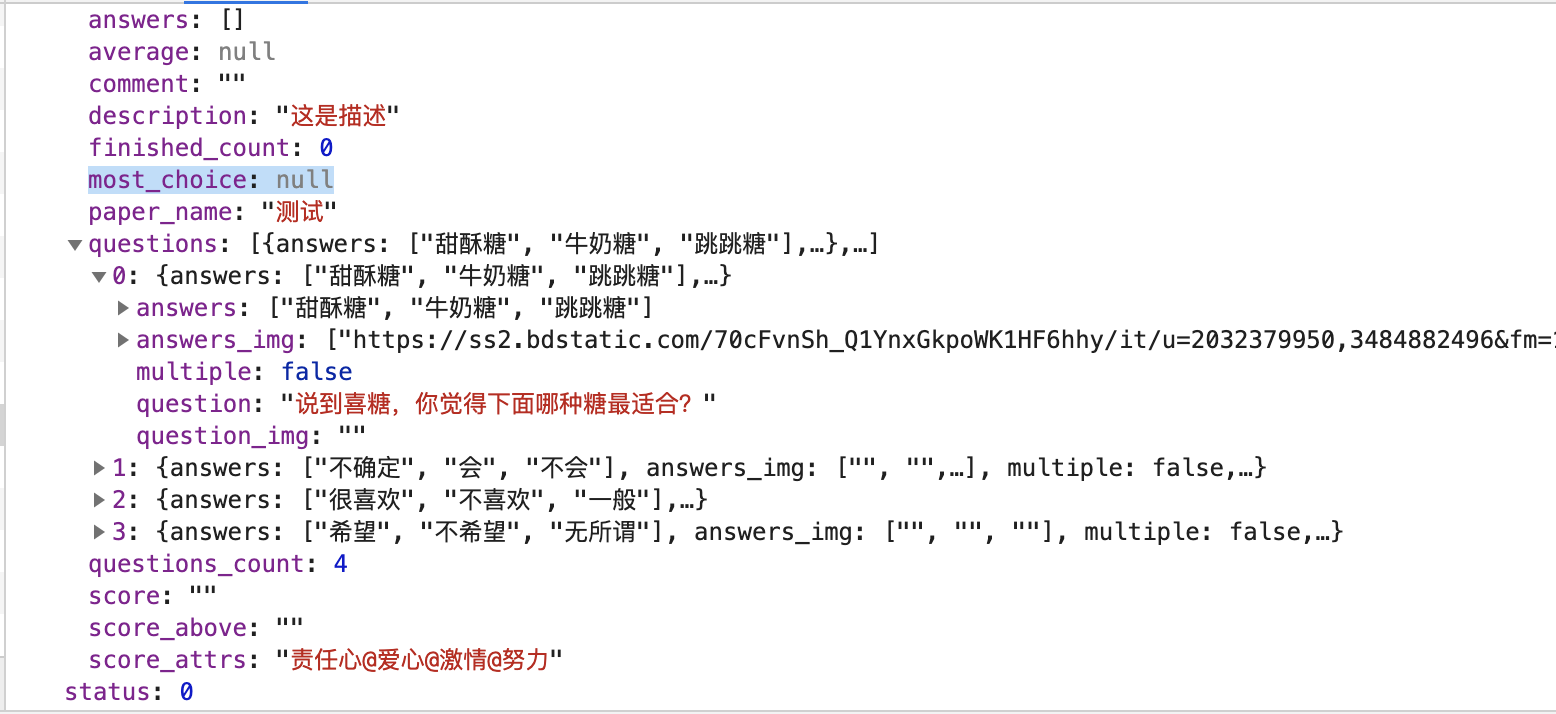
\includegraphics[width=1.0\linewidth]{figure/paper_data}
	\label{fig:paper_data} \\
		图4.7 试卷数据结构
\end{figure}

其中average、comment、most\_choices、answers、score、score\_above、score\_attrs是完成试卷以后才会有的参数,与数据分析结果的接口是一个接口。

\subsubsection{数据分析}

成绩数据表如图4.8所示

\begin{figure}[thbp!]
	\centering
	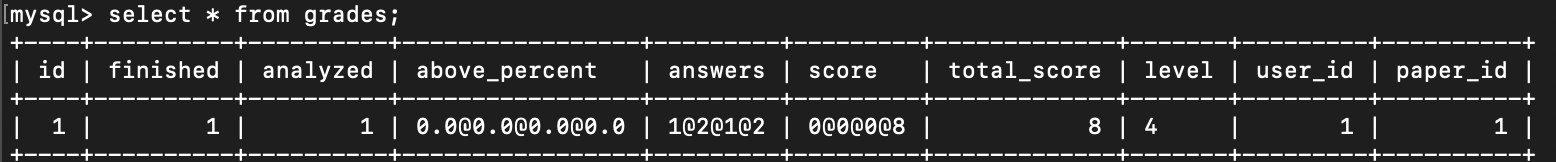
\includegraphics[width=1.0\linewidth]{figure/grade}
	\label{fig:grade} \\
		图4.8 成绩数据表
\end{figure}

用户回答完后,答案之间以"@"分隔开来进行存储。在计算得分的时候遍历答案进行指标的加减。

\subsubsection{计算每个问题最多回答的答案}

计算最多回答的答案的简略代码:

\begin{lstlisting}[language=C]
most_choice = "@".join(map(lambda x: Counter(x)
.most_common(1)[0][0], choices))
\end{lstlisting}

Counter是Python内置的一个计数器类,可以得到每个元素出现的次数,其中.most\_common函数可以得到列表中出现频率最频繁的元素。
